\documentclass[beamer]{beamer}
%\documentclass[handout]{beamer}

\usepackage[english]{babel}
\usepackage[utf8]{inputenc}

\newif\ifconference
\newif\ifoneauthor

%\conferencetrue % or
\conferencefalse
\oneauthortrue %or
%\oneauthorfalse

\usepackage[ruled,vlined,linesnumbered]{algorithm2e}
\SetKwRepeat{Do}{do}{while}

\usepackage{tikz}
\usepackage{pdfrender}
\usepackage[absolute,overlay]{textpos}
% ********** to whom **********

\DeclareUnicodeCharacter{00A0}{ }
%eliminar margen
\newcommand\Wider[2][3em]{%
	\makebox[\linewidth][c]{%
		\begin{minipage}{\dimexpr\textwidth+#1\relax}
			\raggedright#2
		\end{minipage}%
	}%
}

\usepackage{beamerthemeshadow}
\usetheme[blackblocktext,nobg,pagenumbers,nocol]{Dresden}

\definecolor{beamer@personal0}{rgb}{0.780,0.780,0.520}
\definecolor{beamer@personal1}{rgb}{0.600,0.600,0.400}
\definecolor{beamer@personal2}{rgb}{0.540,0.540,0.360}
\definecolor{beamer@personal3}{rgb}{0.420,0.420,0.280}
\definecolor{beamer@personal4}{rgb}{0.360,0.360,0.240}
%\definecolor{beamer@personal2}{rgb}{0.600,0.600,0.400}
%\definecolor{beamer@personal1}{rgb}{0.660,0.660,0.440}

\setbeamercolor{block title}{bg=beamer@personal2,fg=white}
\setbeamercolor{block body}{bg=beamer@personal1,fg=white}
\setbeamercolor{block title example}{bg=beamer@personal2,fg=white}
%\setbeamercolor{block body example}{bg=beamer@personal0,fg=black}


\setbeamertemplate{navigation symbols}{}
\setbeamertemplate{blocks}[rounded]% [shadow=false]

\setbeamercolor*{palette secondary}{use=structure,fg=white,bg=beamer@personal1}
\setbeamercolor*{palette tertiary}{use=structure,fg=white,bg=beamer@personal2}

%Amplío el tamaño de los contenidos
\setbeamertemplate{itemize/enumerate body begin}{\large}
\setbeamertemplate{itemize/enumerate subbody begin}{\large}

%en listas
\setbeamercolor{item projected}{bg=beamer@personal1}
\setbeamercolor{subitem projected}{bg=beamer@personal1}

%en figuras
\setbeamercolor{caption name}{fg=beamer@personal2}

%\setbeamertemplate{itemize item}[\color{beamer@personal1}ball]
%\setbeamertemplate{itemize subitem}{\color{beamer@personal1}$\blacktriangleright$}


%Table of contents 
\setbeamerfont{section in toc}{size=\Large}
\setbeamercolor{section in toc}{fg=black}
\setbeamertemplate{sections/subsections in toc}{ \inserttocsectionnumber.~\inserttocsection}

%change margins (latex margins are a little too generous)
\setbeamersize{text margin left=0.75cm,text margin right=1cm} 

%eliminar shadow from titles
\setbeamerfont{frametitle}{size=\LARGE}
\setbeamertemplate{frametitle}{%
	\nointerlineskip%
	\begin{beamercolorbox}[wd=\paperwidth,ht=2.5ex,dp=0.6ex]{frametitle}
		\hspace*{2ex} \insertframetitle %
	\end{beamercolorbox}%
}

\ifoneauthor
\setbeamerfont{author}{size=\fontsize{14}{16}}
\else
\setbeamerfont{author}{size=\fontsize{12}{14}}
\fi
\setbeamerfont{institute}{size=\normalsize\itshape}
\setbeamerfont{title}{size=\fontsize{19}{21}}
\setbeamerfont{subtitle}{size=\Large\normalfont\slshape}

%modificamos pagina de title (dibujo chulo)
\setbeamertemplate{title page}{%
	\begin{tikzpicture}[remember picture,overlay]
	\fill[beamer@personal1]
	([yshift=-5pt]current page.west) rectangle (current page.south east);
	\node[anchor=east] 
	at ([yshift=-70pt]current page.north east) (author)
	{\parbox[t]{.9\paperwidth}{\raggedleft%
			\usebeamerfont{author}\textcolor{beamer@personal2}{%
				\textpdfrender{
					TextRenderingMode=FillStroke,
					FillColor=beamer@personal2,
					LineWidth=.1ex,
				}{\insertauthor}}}};
	\node[anchor=north east] 
	at ([yshift=-80pt]current page.north east) (institute)
	{\parbox[t]{.78\paperwidth}{\raggedleft%
			\usebeamerfont{institute}\textcolor{beamer@personal2}{\insertinstitute}}};
	\node[anchor=south west] 
	at ([yshift=26pt,xshift=15pt]current page.west) (logo)
	{\parbox[t]{.19\paperwidth}{\raggedleft%
			\usebeamercolor[fg]{titlegraphic}\inserttitlegraphic}};
	\node[anchor=east]
	at ([yshift=-50pt,xshift=-20pt]current page.east) (title)
	{\parbox[t]{\textwidth}{\raggedleft%
			\usebeamerfont{title}\textcolor{white}{%
				\textpdfrender{
					TextRenderingMode=FillStroke,
					FillColor=white,
					LineWidth=.1ex,
				}{\inserttitle}}}};
	\node[anchor=east]
	at ([yshift=-80pt,xshift=-20pt]current page.east) (subtitle)
	{\parbox[t]{\paperwidth}{\raggedleft\usebeamerfont{subtitle}\textcolor{white}{\insertsubtitle}}};
	\end{tikzpicture}
}

% different headline
\setbeamertemplate{headline}
{%
	\begin{beamercolorbox}[colsep=0pt]{upper separation line head}
	\end{beamercolorbox}
	\begin{beamercolorbox}{section in head/foot} %
		\vskip2pt\insertnavigation{\paperwidth}\vskip5pt
	\end{beamercolorbox}%
	%\begin{beamercolorbox}[colsep=-0pt]{lower separation line head}
	%\end{beamercolorbox}
}

% different footnote
\setbeamertemplate{footline}
{
	\leavevmode%
	\hbox{
		\begin{beamercolorbox}[wd=1.1\paperwidth,ht=2.25ex,dp=1ex,center]{title in head/foot}%
			\usebeamerfont{title in head/foot}\insertshorttitle
		\end{beamercolorbox}%
	}
}


% logos
\ifconference
\titlegraphic{
\includegraphics[width=2.5cm]{cplex}}
\else
\titlegraphic{
\includegraphics[width=4.5cm]{figuras/cplex}}
\fi
	

\title{Uso de CPLEX junto a Excel}
\subtitle[]{Varias alternativas} 
\author[J.\ Pereira]{Jordi Pereira}
\date[]{5 de enero del 2018}

\institute[UAI]{Faculty of Engineering and Sciences\\
  Universidad Adolfo Ib\'{a}\~{n}ez,\\
  Vi\~{n}a del Mar, Chile}

\begin{document}

	%título
	\begin{frame}[plain]
		\maketitle
	\end{frame}
	
	%table of contents
	\begin{frame}\frametitle{Contenidos}\tableofcontents
	\end{frame} 


\section{Introducción} 
\subsection{}

\frame[t]{ % Broad definition of a packing problem
	\frametitle{Diferentes opciones}
	\vfill
	\begin{itemize}\itemsep2ex
		\item Hay diferentes maneras de asociar Cplex y Excel dependiendo del objetivo buscado.
		\item Veremos aquí varias maneras que van desde la sustitución del Solver de Excel por Cplex hasta referirse a Excel como una fuente de entrada y salida de datos. 
		\item Alguna de las opciones que mostraremos requiere cierto conocimiento de programación
		\item IBM ha ido dejando de ofrecer soporte para alguna de las opciones que veremos (específicamente llamar a Cplex desde Excel).
	\end{itemize}
}

\frame[t]{ % Broad definition of a packing problem
	\frametitle{Modelos}
	A lo largo de los ejemplos veremos dos modelos diferentes que servirán para ilustrar el proceso de modelización y resolución mediante Cplex. Los modelos que veremos son dos problemas clásicos del área:

	\begin{itemize}
		\item Uncapacitated Lot Sizing Problem
		\item Set Covering Problem
	\end{itemize}

	\vfill
	
	Vamos a ver una formulación de cada problema.

}

\frame[t]{ % Broad definition of a packing problem
	\frametitle{Uncapacitated Lot Sizing}
	Modelo estándar de inventarios con demanda determinista y heterogénea en $T$ periodos. 
		
\begin{align*}
\min & ~\sum_{t=1}^{T} c_l y_t + \sum_{t=1}^{T} c_s s_t & \\
\mbox{s.t.} & \\
& x_t + s_{t-1} = d_t + s_t & & 1\leq t \leq T; \\
& x_t \leq \mbox{M} y_t & & 1\leq t\leq T; \\ 
& s_0 = 0 & & \\
& y_t  \in \{0,1\},~x_{t} \geq 0,~s_t \geq 0 & & 1\leq t\leq T.
\end{align*}
	
}

\frame[t]{ % Broad definition of a packing problem
	\frametitle{Set Covering}
	Cubrimiento de conjuntos y subproblema de otros modelos más complejos (itinerarios, localización, \emph{timetabling},...). 
	
	\begin{align*}
	\min & ~\sum_{i=1}^{n} c_i x_i & \\
	\mbox{s.t.} & \\
	& \sum_{i=1}^{n} a_{ij} x_i \geq 1 & & 1\leq j \leq m; \\
	& x_i  \in \{0,1\} & & 1\leq i\leq n.
	\end{align*}
	
}

\section{Cplex+Excel} 
\subsection{}

\frame[t]{ % Introducción CPLEX+excel
	\frametitle{Introducción}
	
	\textbf{Pros:}

		\begin{itemize}\itemsep1ex
		\item A priori, la forma más sencilla de hacer las cosas.
		\item Cplex sustituye a Excel Solver utilizando un interfaz muy similar al del segundo.
		\item Puede incluso llamarse desde una macro.
		\end{itemize}

	\textbf{Contras:}

		\begin{itemize}\itemsep1ex
		\item IBM ya no ofrece soporte para este método (esta opción ya no existe en Cplex 12.7 ni Cplex 12.8, además el módulo dejó de desarrollarse en Excel 2010).
		\item En pocas palabras: \emph{``Use at your own risk"} a sabiendas que tarde o temprano dejará de funcionar según se vayan actualizando los equipos.
		\end{itemize}
}

\frame[t]{ % Cplex
	\frametitle{Activando Cplex en Excel}
	
	Tenemos que activar un módulo en Excel (menú Opciones). 
			\begin{figure}
	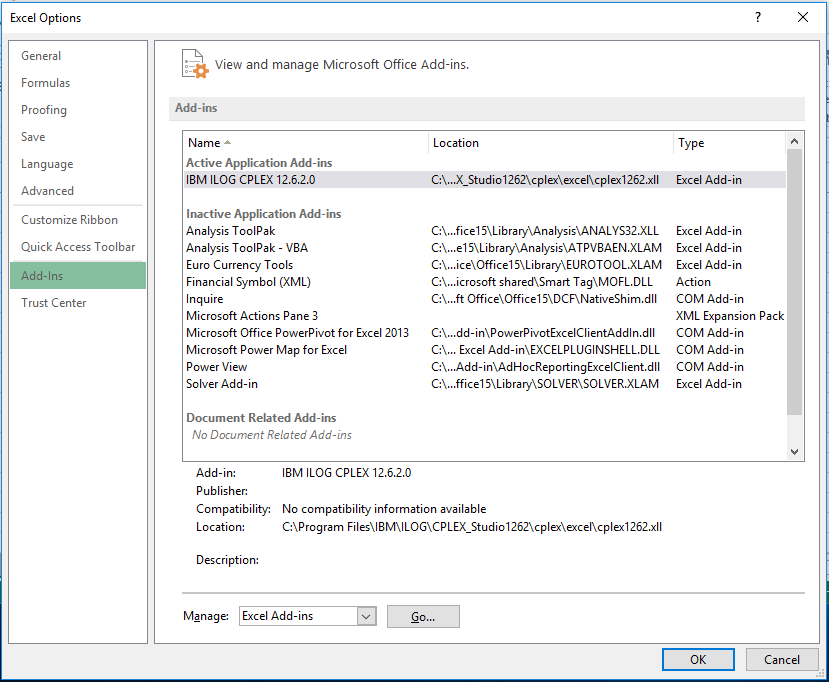
\includegraphics[width=0.7\textwidth]{figuras/corte1}
\end{figure}

}

\frame[t]{ % VBA
	\frametitle{Activando VBA}
	
	Tenemos que mostrar las opciones de desarrollo. 
	\begin{figure}
		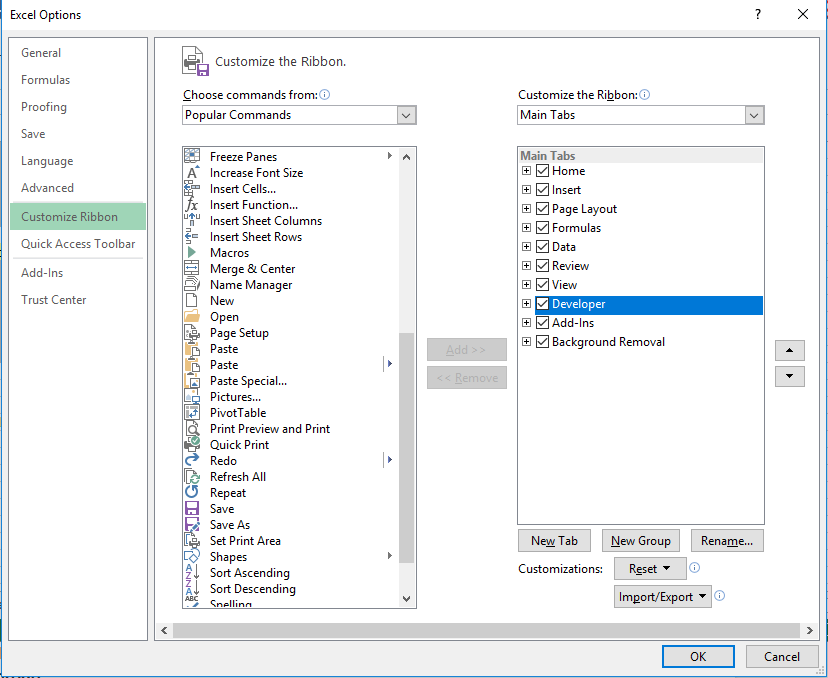
\includegraphics[width=0.7\textwidth]{figuras/corte2}
	\end{figure}
	
}

\frame[t]{ % VBA
	\frametitle{Usar Cplex}
	
	Usar Cplex como sustituto de Solver requiere de los mismos pasos que usaríamos con Solver. 

	\vfill

	\begin{enumerate}
		\item Construir la hoja de cálculo
		\item Determinar las variables (casillas)
		\item Determinar la función objetivo (casilla)
		\item Construir el lado izquierdo y derecho de las restricciones
	\end{enumerate}
	
	\vfill
	
	Puede haber algunos ``problemillas" de uso.
}

\frame[t]{ % Ejemplo 1
	\frametitle{Ejemplo ULS}
	
	\only<1>
	{
		Podemos descargar la hoja de cálculo inicial para hacer el ejercicio de \href{https://github.com/jordipereiragude/ExcelwithCplex/blob/master/workbooks/uls_empty.xlsx}{goo.gl/n919co}
	}
	\only<2>
	{		
		La versión finalizada puede descargarse de \href{https://github.com/jordipereiragude/ExcelwithCplex/blob/master/workbooks/uls.xlsx}{goo.gl/xyVyzr}	
	}
	\begin{figure}
	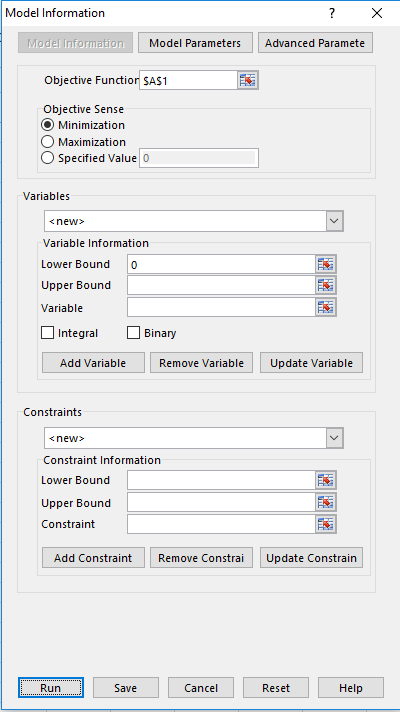
\includegraphics[width=0.30\textwidth]{figuras/corte3}
	\end{figure}
	
}

\frame[t]{ % Ejemplo 2
	\frametitle{Ejemplo SCP (versión 1)}
	
	\begin{itemize}\itemsep1ex
	\item De forma parecida al caso anterior, podemos resolver el modelo de cubrimiento. Descargar hoja de cálculo de \href{https://github.com/jordipereiragude/ExcelwithCplex/blob/master/workbooks/scp_empty.xlsx}{goo.gl/8M46Ry} y de \href{https://github.com/jordipereiragude/ExcelwithCplex/blob/master/workbooks/scp.xlsx}{goo.gl/fFw9Tj} para la hoja completa. 
	\item En este caso podemos visualizar que la técnica anterior no escala bien para problemas grandes ni formulaciones en que la matriz $A$ está formada mayoritariamente por entradas iguales 0 (lo que se entiende como una matriz dispersa).
	\item Aquí es cuando se aprecia la oportunidad de mejorar el flujo de trabajo construyendo el modelo de forma programática.
	\end{itemize}
}

\frame[t]{ % Ejemplo 2
	\frametitle{Utilizando macros}

	\begin{itemize}\itemsep1ex
		\item	Generalmente, la información del modelo anterior se hubiera entregado como una lista de costos y otra de no-ceros.
		\item Partiendo de esas listas podemos construir el modelo matemático.
		\item Vamos a usar macros de Excel (lenguaje Visual Basic for Applications).
	\end{itemize}
\vfill

	No se preocupen, pueden bajar el archivo directamente (\href{https://github.com/jordipereiragude/ExcelwithCplex/blob/master/workbooks/scp-vba.xlsm}{goo.gl/6v72sD}) y podemos analizar el código paso a paso.
}

\frame[t]{ % Ejemplo 2
	\frametitle{Ejemplo SCP (versión 2)}

	\begin{textblock*}{\paperwidth}(0in,0.5in)
	\begin{figure}
	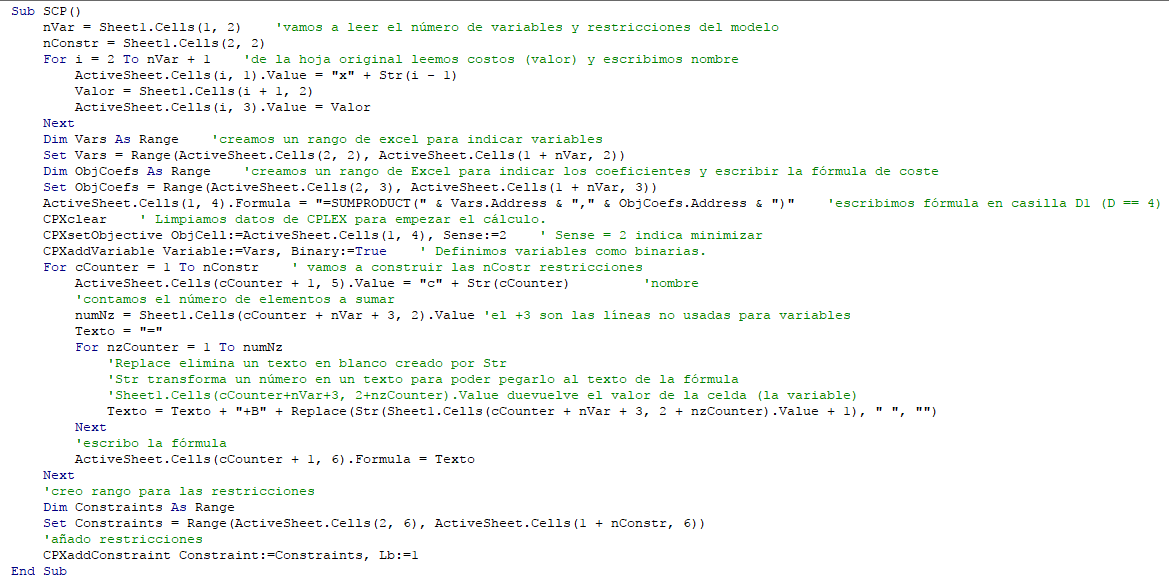
\includegraphics[width=1\textwidth]{figuras/corte4}
	\end{figure}
	\end{textblock*}
}


\section{OPL+Excel} 
\subsection{}
\frame[t]{ %Truncated enumeration [1]
	\frametitle{Introducción}

	\textbf{Pros:}

\begin{itemize}\itemsep1ex
	\item Es la forma recomendada por IBM.
	\item Puede integrarse de forma ``profesional" (a costa de programar un poco).
	\item Proporciona un modelizador.
\end{itemize}

\textbf{Contras:}

\begin{itemize}\itemsep1ex
	\item La curva de aprendizaje es un poco mayor.
	\item El trabajo se hace fuera de Excel.
\end{itemize}
}

\frame[t]{ %Modus operandi
		\frametitle{Modus Operandi}
			
	\begin{textblock*}{\paperwidth}(0in,0.5in)
	\begin{figure}
		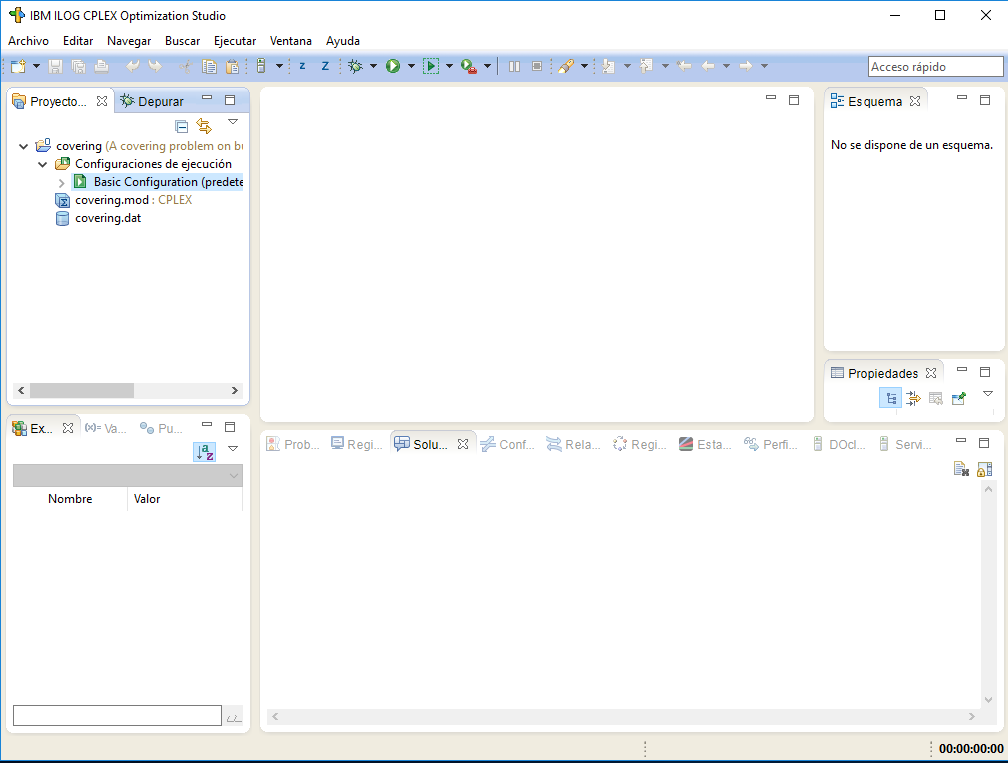
\includegraphics[height=0.85\textheight]{figuras/corte5}
	\end{figure}
	\end{textblock*}

	\begin{textblock*}{0.25\paperwidth}(0.25in,1.6in)
		Archivos abiertos en editor
	\end{textblock*}

	\begin{textblock*}{0.25\paperwidth}(2in,1.6in)
	Editor de textos
\end{textblock*}

	\begin{textblock*}{0.25\paperwidth}(2in,2.6in)
	Resultados e información de ejecución
	\end{textblock*}

	\begin{textblock*}{0.25\paperwidth}(3.8in,1.4in)
	Elementos del modelo encontrados
	\end{textblock*}

}


\frame[t]{ %Modus operandi
	\frametitle{Entorno de trabajo}
	
	\begin{itemize}\itemsep1ex
		\item OPL estructura la información en dos partes: \textbf{Modelo} y \textbf{Datos}. 
		\item La parte de modelo se divide en tres partes: lectura de datos, modelo matemático (las ecuaciones) y escritura de datos
		\item La fuente de datos para la lectura y escritura son un archivo de texto (por defecto)
		\item Haremos que el archivo de texto sea una hoja de Excel.
	\end{itemize}
	Podemos descargar un zip con todos los archivos necesarios de \href{https://github.com/jordipereiragude/ExcelwithCplex/blob/master/workbooks/uls_opl.zip}{http://goo.gl/oSWy1M}
}

\frame[t]{ %Modus operandi
	\frametitle{Código del modelo (independiente del archivo)}
	\begin{textblock*}{\paperwidth}(0in,0.5in)
	\begin{figure}
		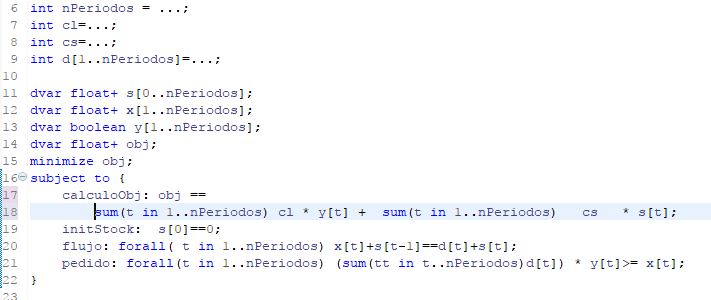
\includegraphics[height=0.65\textheight]{figuras/corte6}
	\end{figure}
\end{textblock*}
}

\frame[t]{ %Modus operandi
	\frametitle{Entrada y salida del modelo}
	\begin{textblock*}{\paperwidth}(0in,0.5in)
		\begin{figure}
			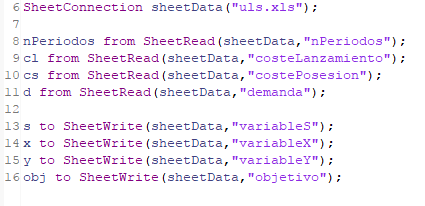
\includegraphics[height=0.6\textheight]{figuras/corte7}
		\end{figure}
	\end{textblock*}

	\begin{textblock*}{0.85\paperwidth}(0.25in,3in)
		Vayan con cuidado, es necesario que el archivo Excel esté cerrado
	\end{textblock*}
}

\frame[t]{ %Modus operandi
	\frametitle{Nombres en Excel}
	
	Hemos tenido que poner nombres a las casillas en Excel. Esto se puede conseguir usando el botón derecho y escogiendo el nombre. Así hemos definido las zonas para la solución y la lectura de datos:
	
	\begin{itemize}
		\item nPeriodos
		\item costeLanzamiento
		\item costePosesion
		\item demanda
		\item variableX, variableY, variableS,objetivo
	\end{itemize}
}

\frame[t]{ %Modus operandi
	\frametitle{Ejercicio}
	
	Hagamos el mismo proceso con el problema de cubrimiento.
	
}


\section{JuMP (+Excel)}
 
\subsection{}
\frame[t]{ %Truncated enumeration [1]
	\frametitle{Introducción}
	
	\begin{itemize}
	\item Personalmente no uso ninguna de las soluciones anterioress.
	\item Recientemente han aparecido diversas opciones para facilitar el trabajo con modelos matemáticos.
	\item Mi favorita es Julia/JuMP. No es exactamente una forma de trabajar con Excel y Cplex pero puede integrarse con las anteriores.	
	\end{itemize}	

\textbf{Pros:}
	\begin{itemize}
		\item Lenguaje moderno completo.
		\item Un modelizador que integra directamente con el lenguaje (importante para usar algoritmos ``complejos" como branch and cut, Dantzig-Wolfe,...).
		\item ``Solver agnostic".
		\item Podemos practicar sin necesidad de tener instalado un solver.
	\end{itemize}

}

\frame[t]{ %Truncated enumeration [1]
	\frametitle{Online}
	
	Podemos ejecutar Julia desde una página web utilizando \href{www.juliabox.com}{www.juliabox.com} y una cuenta google (o ucn.cl)
	
		\begin{textblock*}{\paperwidth}(0in,1.5in)
		\begin{figure}
			
\includegraphics[width=0.5\textwidth]{figuras/juliacloudlogo}
		\end{figure}
	\end{textblock*}
}

\frame[t]{ %Truncated enumeration [1]
	\frametitle{Offline}
	
	\begin{itemize}
	\item Podemos ejecutar Julia de varias maneras (línea de comando, Jupyter local, Juno ...)
	\item Podemos ejecutar diferentes solvers de programación lineal (Cplex, Gurobi, GLPK) cambiando únicamente una línea del archivo.
	\end{itemize}

	\begin{itemize}
		\item Los primeros ejemplos lo vamos a hacer desde Jupyter local.  	Descargar un ejemplo simple de \href{https://raw.githubusercontent.com/jordipereiragude/ExcelwithCplex/master/workbooks/Ejemplo-Simple-JuMP.ipynb}{goo.gl/4yFCwM}
	\end{itemize}
}

\frame[t]{ %Truncated enumeration [1]
	\frametitle{Modelo ``as-is"}

	\begin{textblock*}{\paperwidth}(0in,0.5in)
	\begin{figure}
		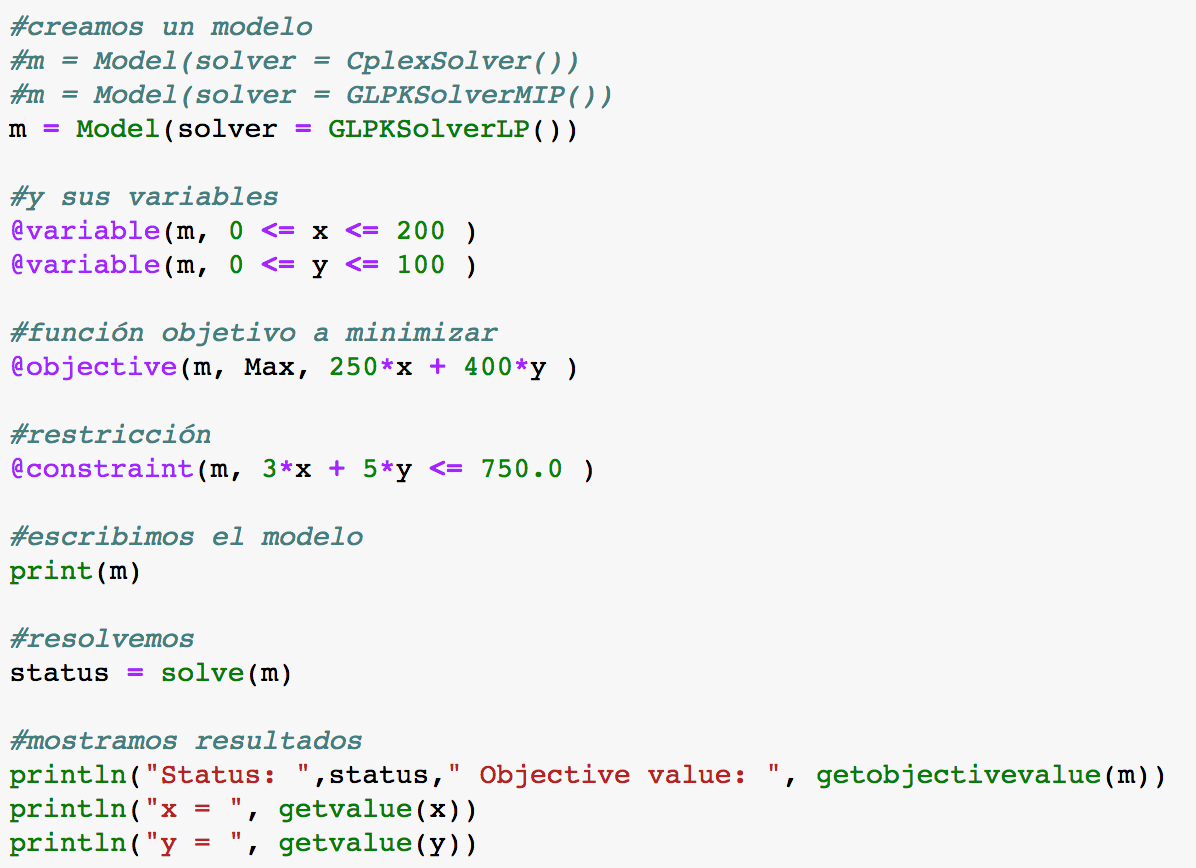
\includegraphics[height=0.85\textheight]{figuras/corte8}
	\end{figure}
\end{textblock*}
	
}

\frame[t]{ %Truncated enumeration [1]
	\frametitle{Modelo inventarios}

Descargar de \href{https://raw.githubusercontent.com/jordipereiragude/ExcelwithCplex/master/workbooks/ULS.ipynb}{goo.gl/DzTY8v}

	\begin{textblock*}{\paperwidth}(0in,0.75in)
		\begin{figure}
			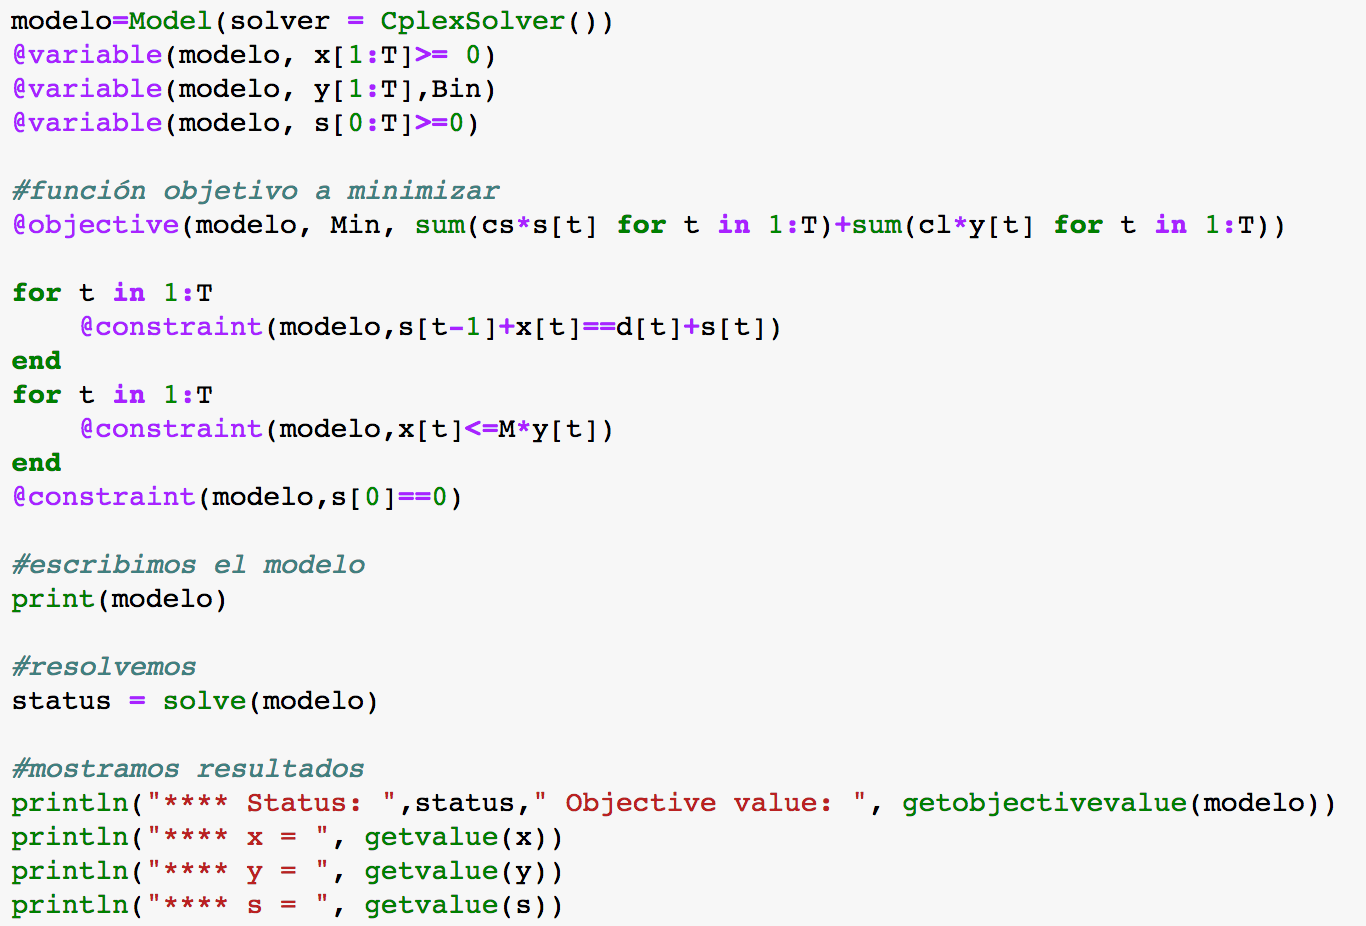
\includegraphics[height=0.8\textheight]{figuras/corte9}
		\end{figure}
	\end{textblock*}
	
}

\frame[t]{ %Truncated enumeration [1]
	\frametitle{Integración con Excel}
	
	Podemos trabajar directamente desde Excel para ello:
	
	\begin{itemize}
	\item Escribir la rutina en un archivo .jl
	\item Crear la macro que llama el archivo .jl
	\item Leer el archivo generado por julia y guardarlo en la hoja de Excel
	\end{itemize}

	\textbf{El paso más complejo es personalizar las rutas hacia y desde los archivos}. El problema es algo tedioso pero no difícil. 
	
	Por si acaso el excel (\href{https://github.com/jordipereiragude/ExcelwithCplex/blob/master/workbooks/uls_juliaDentroExcel.xlsm}{goo.gl/UHE9Dn}) y el archivo julia (\href{https://raw.githubusercontent.com/jordipereiragude/ExcelwithCplex/master/workbooks/uls.jl}{goo.gl/gj9zZw})
} 
\end{document}
